%% Source of figures/mcp-request-lifecycle.pdf (rules/04-figures-tables.md).
%% Build: xelatex -output-directory=figures figures/src/mcp-request-lifecycle.tex
%% Drawn from opentrading-mcp de956f8: cli.py build_http_app, middleware.py, tools/shared.py,
%% providers/circuit.py, providers/pool.py, units.py.
\documentclass[border=2pt]{standalone}
\usepackage{fontspec}
\IfFontExistsTF{Arial}{\setmainfont{Arial}}{\setmainfont{TeX Gyre Heros}}
\usepackage{tikz}
\usetikzlibrary{positioning,arrows.meta,fit,backgrounds}
\begin{document}
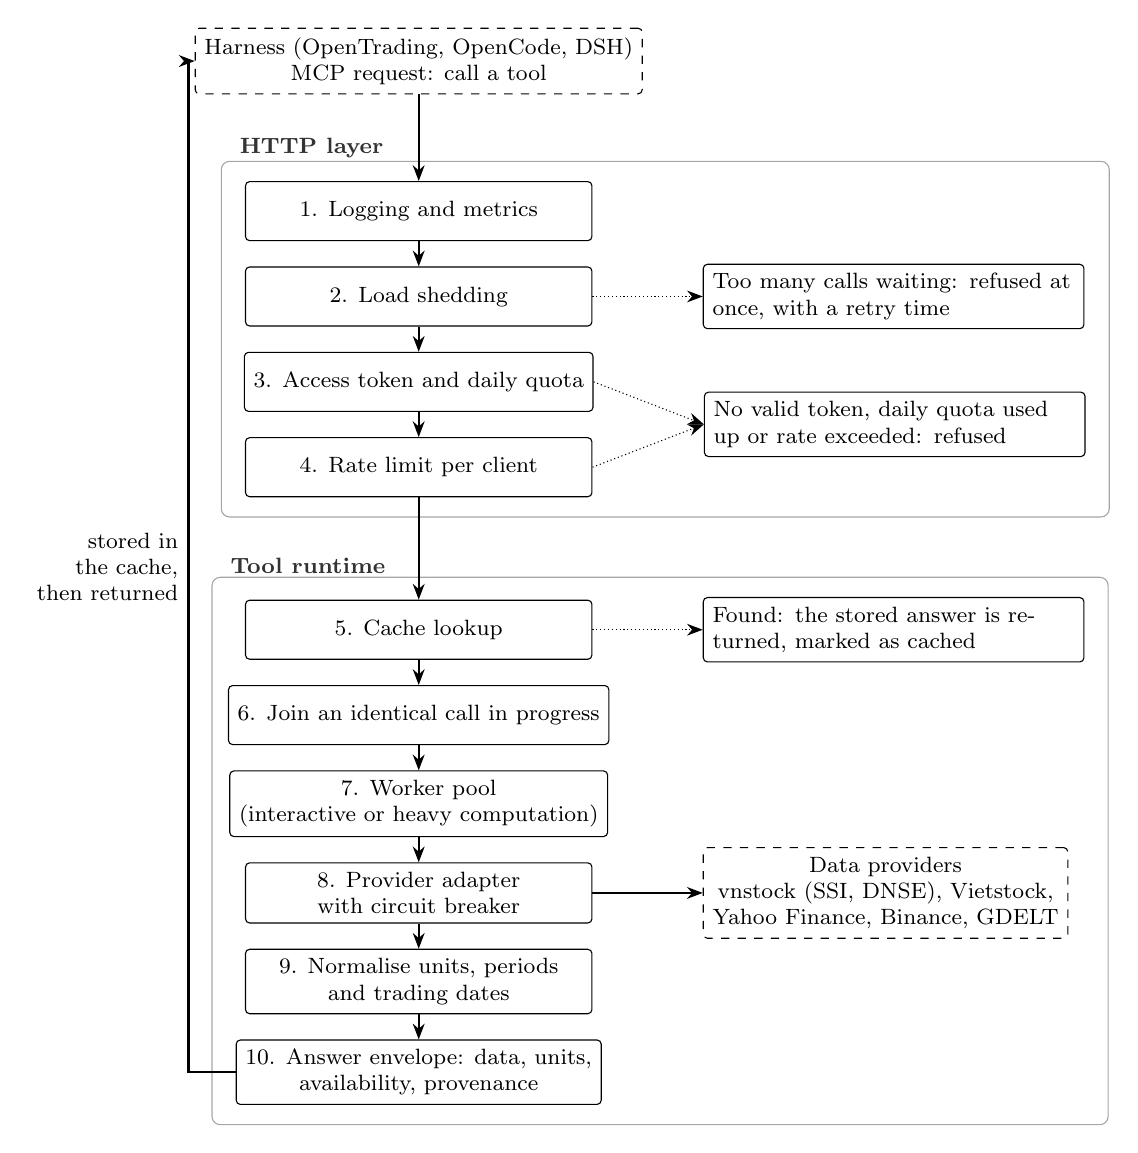
\begin{tikzpicture}[
  font=\fontsize{8}{9.5}\selectfont,
  node distance=3.2mm and 6mm,
  box/.style={draw, rounded corners=1.5pt, align=center, minimum width=44mm, minimum height=7.5mm, fill=white},
  side/.style={draw, rounded corners=1.5pt, align=left, text width=46mm, minimum height=7.5mm, fill=white},
  ext/.style={box, dashed},
  arr/.style={-{Stealth[length=2mm]}, thick},
  side arrow/.style={-{Stealth[length=2mm]}, densely dotted},
  group/.style={draw, gray!70, rounded corners=3pt, inner xsep=3mm, inner ysep=2.5mm},
  glabel/.style={font=\fontsize{8}{9.5}\selectfont\bfseries, anchor=south west, gray!40!black, inner sep=1pt}
]
\node[ext] (client) {Harness (OpenTrading, OpenCode, DSH)\\MCP request: call a tool};

\node[box, below=11mm of client] (obs) {1. Logging and metrics};
\node[box, below=of obs] (shed) {2. Load shedding};
\node[box, below=of shed] (auth) {3. Access token and daily quota};
\node[box, below=of auth] (rate) {4. Rate limit per client};

\node[box, below=13mm of rate] (cache) {5. Cache lookup};
\node[box, below=of cache] (flight) {6. Join an identical call in progress};
\node[box, below=of flight] (pool) {7. Worker pool\\(interactive or heavy computation)};
\node[box, below=of pool] (prov) {8. Provider adapter\\with circuit breaker};
\node[box, below=of prov] (norm) {9. Normalise units, periods\\and trading dates};
\node[box, below=of norm] (env) {10. Answer envelope: data, units,\\availability, provenance};

\node[ext, right=14mm of prov] (up) {Data providers\\vnstock (SSI, DNSE), Vietstock,\\Yahoo Finance, Binance, GDELT};

\node[side, right=14mm of shed] (busy) {Too many calls waiting: refused at once, with a retry time};
\node[side, right=14mm of auth, yshift=-5.4mm] (deny) {No valid token, daily quota used up or rate exceeded: refused};
\node[side, right=14mm of cache] (hit) {Found: the stored answer is returned, marked as cached};

\draw[arr] (client) -- (obs);
\foreach \a/\b in {obs/shed, shed/auth, auth/rate, rate/cache, cache/flight, flight/pool, pool/prov, prov/norm, norm/env}
  \draw[arr] (\a) -- (\b);
\draw[arr] (prov.east) -- (up.west);
\draw[side arrow] (shed.east) -- (busy.west);
\draw[side arrow] (auth.east) -- (deny.west);
\draw[side arrow] (rate.east) -- (deny.west);
\draw[side arrow] (cache.east) -- (hit.west);
\draw[arr] (env.west) -- ++(-6mm,0) |- node[pos=0.25, left, align=right] {stored in\\the cache,\\then returned} (client.west);

\begin{scope}[on background layer]
  \node[group, fit=(obs)(rate)(busy)(deny)] (http) {};
  \node[glabel] at ([xshift=2mm]http.north west) {HTTP layer};
  \node[group, fit=(cache)(env)(hit)(up)] (rt) {};
  \node[glabel] at ([xshift=2mm]rt.north west) {Tool runtime};
\end{scope}
\end{tikzpicture}
\end{document}
